% 20_arbol_pruebas.tex: árbol de decisión para elegir la prueba de contraste
% (standalone; TikZ choca con ctable en la presentación) -> img/arbol_pruebas.pdf
\documentclass[border=3pt]{standalone}
\usepackage[utf8]{inputenc}
\usepackage{mathpazo}
\usepackage{tikz}
\usetikzlibrary{trees,positioning}
\begin{document}
\footnotesize
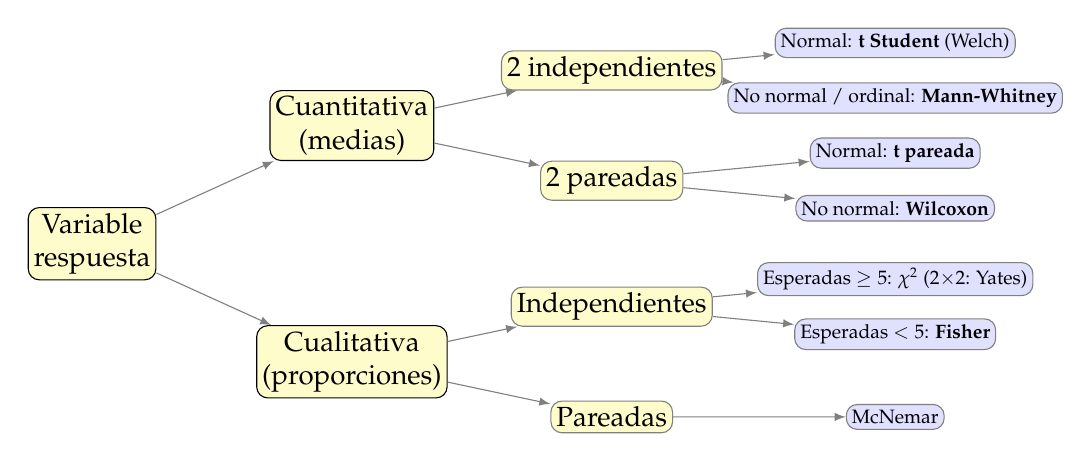
\begin{tikzpicture}[
  grow=right, level distance=33mm,
  level 1/.style={sibling distance=30mm},
  level 2/.style={sibling distance=14mm},
  level 3/.style={sibling distance=7mm, level distance=36mm},
  caja/.style={draw, rounded corners, fill=yellow!20, align=center, inner sep=2pt},
  prueba/.style={draw, rounded corners, fill=blue!12, align=left, inner sep=2pt, font=\scriptsize},
  edge from parent/.style={draw, -latex, gray}]
\node[caja]{Variable\\respuesta}
  child{node[caja]{Cualitativa\\(proporciones)}
    child{node[caja]{Pareadas}
      child{node[prueba]{McNemar}}}
    child{node[caja]{Independientes}
      child{node[prueba]{Esperadas $<5$: \textbf{Fisher}}}
      child{node[prueba]{Esperadas $\geq5$: \textbf{$\chi^2$} (2$\times$2: Yates)}}}}
  child{node[caja]{Cuantitativa\\(medias)}
    child{node[caja]{2 pareadas}
      child{node[prueba]{No normal: \textbf{Wilcoxon}}}
      child{node[prueba]{Normal: \textbf{t pareada}}}}
    child{node[caja]{2 independientes}
      child{node[prueba]{No normal / ordinal: \textbf{Mann-Whitney}}}
      child{node[prueba]{Normal: \textbf{t Student} (Welch)}}}};
\end{tikzpicture}
\end{document}
